\documentclass[tikz]{standalone}
\usepackage{tikz}
\usepackage[AutoFakeBold=true,AutoFakeSlant=true]{xeCJK}
\usepackage[zihao=-4,UTF8,heading=true]{ctex}
\usepackage[simplified]{pgf-umlcd}
\usetikzlibrary{fit} %形状
\usetikzlibrary{positioning} %不加方向运算可能出错
\usetikzlibrary{arrows.meta} %箭头
\usetikzlibrary{calc}

\setCJKmainfont{微软雅黑}
\begin{document}
	\thispagestyle{empty}
    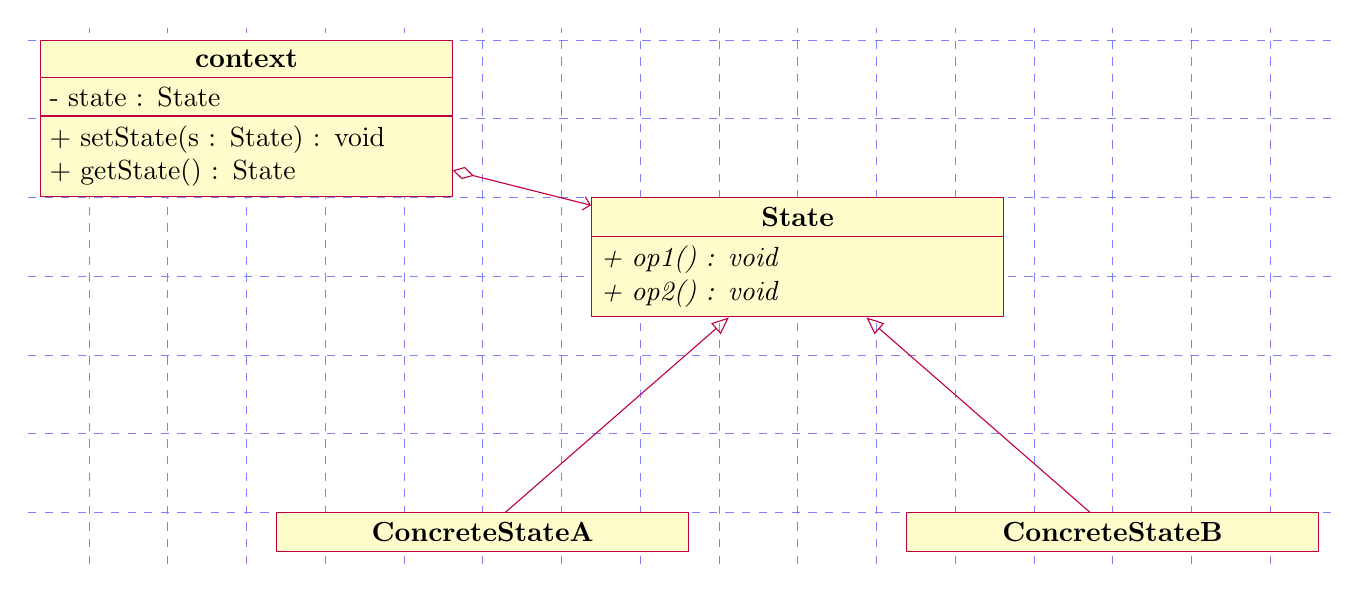
\begin{tikzpicture}[show background grid]
        \begin{class}[text width=5cm]{State}{0,0}
            \operation[0]{+ op1() : void}
            \operation[0]{+ op2() : void}
        \end{class}
        \begin{class}[]{ConcreteStateA}{-4, -4}
            \inherit{State}
        \end{class}
        \begin{class}[]{ConcreteStateB}{4, -4}
            \inherit{State}
        \end{class}
        \begin{class}[]{context}{-7, 2}
            \attribute{- state : State }
            \operation{+ setState(s : State) : void}
            \operation{+ getState() : State }
        \end{class}
        \aggregation{context}{}{}{State}
        
    \end{tikzpicture}

\end{document}